\documentclass[a4paper]{amsart}

\usepackage{amsmath,amsfonts,amssymb,amsthm} %AMS packages
\usepackage{mathrsfs} %Script fonts
\usepackage[shortlabels]{enumitem} %Adds extra options to enumerate environment
\usepackage{caption} %Gives better caption formatting and more caption formatting options
\usepackage[T1]{fontenc} %Extra font characters

\usepackage{mathtools} %Fixes some problems with amsmath and adds some commands
\mathtoolsset{centercolon} %Corrects colons before equals signs

\usepackage{tikz} %TikZ for drawing things
\usetikzlibrary{cd} %Commutative diagrams

\usepackage{pdflscape,multirow}

\usepackage{hyperref} %Hyperlinks

\usepackage{todonotes}

\theoremstyle{definition}
\newtheorem{definition}{Definition}[section]
\newtheorem{assumption}[definition]{Assumption}
\newtheorem{assumptions}[definition]{Assumptions}
\newtheorem{computation}[definition]{Computation}

\theoremstyle{plain}
\newtheorem{lemma}[definition]{Lemma}
\newtheorem{theorem}[definition]{Theorem}
\newtheorem{proposition}[definition]{Proposition}
\newtheorem{corollary}[definition]{Corollary}
\newtheorem{conjecture}[definition]{Conjecture}
\newtheorem{axiom}[definition]{Axiom}

\theoremstyle{remark}
\newtheorem{remark}[definition]{Remark}
\newtheorem{example}[definition]{Example}
\newtheorem{exercise}[definition]{Exercise}

%Bold letters
\newcommand{\ba}{\mathbf{a}}
\newcommand{\bb}{\mathbf{b}}
\newcommand{\bc}{\mathbf{c}}
\newcommand{\bd}{\mathbf{d}}
\newcommand{\be}{\mathbf{e}}
\newcommand{\bff}{\mathbf{f}}
\newcommand{\bg}{\mathbf{g}}
\newcommand{\bh}{\mathbf{h}}
\newcommand{\bi}{\mathbf{i}}
\newcommand{\bj}{\mathbf{j}}
\newcommand{\bk}{\mathbf{k}}
\newcommand{\bl}{\mathbf{l}}
\newcommand{\bm}{\mathbf{m}}
\newcommand{\bn}{\mathbf{n}}
\newcommand{\bo}{\mathbf{o}}
\newcommand{\bp}{\mathbf{p}}
\newcommand{\bq}{\mathbf{q}}
\newcommand{\br}{\mathbf{r}}
\newcommand{\bs}{\mathbf{s}}
\newcommand{\bt}{\mathbf{t}}
\newcommand{\bu}{\mathbf{u}}
\newcommand{\bv}{\mathbf{v}}
\newcommand{\bw}{\mathbf{w}}
\newcommand{\bx}{\mathbf{x}}
\newcommand{\by}{\mathbf{y}}
\newcommand{\bz}{\mathbf{z}}
\newcommand{\bzero}{\mathbf{0}}

%Blackboard bold letters
\newcommand{\bA}{\mathbb{A}}
\newcommand{\bB}{\mathbb{B}}
\newcommand{\bC}{\mathbb{C}}
\newcommand{\bD}{\mathbb{D}}
\newcommand{\bE}{\mathbb{E}}
\newcommand{\bF}{\mathbb{F}}
\newcommand{\bG}{\mathbb{G}}
\newcommand{\bH}{\mathbb{H}}
\newcommand{\bI}{\mathbb{I}}
\newcommand{\bJ}{\mathbb{J}}
\newcommand{\bK}{\mathbb{K}}
\newcommand{\bL}{\mathbb{L}}
\newcommand{\bM}{\mathbb{M}}
\newcommand{\bN}{\mathbb{N}}
\newcommand{\bO}{\mathbb{O}}
\newcommand{\bP}{\mathbb{P}}
\newcommand{\bQ}{\mathbb{Q}}
\newcommand{\bR}{\mathbb{R}}
\newcommand{\bS}{\mathbb{S}}
\newcommand{\bT}{\mathbb{T}}
\newcommand{\bU}{\mathbb{U}}
\newcommand{\bV}{\mathbb{V}}
\newcommand{\bW}{\mathbb{W}}
\newcommand{\bX}{\mathbb{X}}
\newcommand{\bY}{\mathbb{Y}}
\newcommand{\bZ}{\mathbb{Z}}
\newcommand{\WP}{\mathbb{W}\mathbb{P}}

%Calligraphic letters
\newcommand{\calA}{\mathcal{A}}
\newcommand{\calB}{\mathcal{B}}
\newcommand{\calC}{\mathcal{C}}
\newcommand{\calD}{\mathcal{D}}
\newcommand{\calE}{\mathcal{E}}
\newcommand{\calF}{\mathcal{F}}
\newcommand{\calG}{\mathcal{G}}
\newcommand{\calH}{\mathcal{H}}
\newcommand{\calI}{\mathcal{I}}
\newcommand{\calJ}{\mathcal{J}}
\newcommand{\calK}{\mathcal{K}}
\newcommand{\calL}{\mathcal{L}}
\newcommand{\calM}{\mathcal{M}}
\newcommand{\calN}{\mathcal{N}}
\newcommand{\calO}{\mathcal{O}}
\newcommand{\calP}{\mathcal{P}}
\newcommand{\calQ}{\mathcal{Q}}
\newcommand{\calR}{\mathcal{R}}
\newcommand{\calS}{\mathcal{S}}
\newcommand{\calT}{\mathcal{T}}
\newcommand{\calU}{\mathcal{U}}
\newcommand{\calV}{\mathcal{V}}
\newcommand{\calW}{\mathcal{W}}
\newcommand{\calX}{\mathcal{X}}
\newcommand{\calY}{\mathcal{Y}}
\newcommand{\calZ}{\mathcal{Z}}

%Roman letters
\newcommand{\rmA}{\mathrm{A}}
\newcommand{\rmB}{\mathrm{B}}
\newcommand{\rmC}{\mathrm{C}}
\newcommand{\rmD}{\mathrm{D}}
\newcommand{\rmE}{\mathrm{E}}
\newcommand{\rmF}{\mathrm{F}}
\newcommand{\rmG}{\mathrm{G}}
\newcommand{\rmH}{\mathrm{H}}
\newcommand{\rmI}{\mathrm{I}}
\newcommand{\rmJ}{\mathrm{J}}
\newcommand{\rmK}{\mathrm{K}}
\newcommand{\rmL}{\mathrm{L}}
\newcommand{\rmM}{\mathrm{M}}
\newcommand{\rmN}{\mathrm{N}}
\newcommand{\rmO}{\mathrm{O}}
\newcommand{\rmP}{\mathrm{P}}
\newcommand{\rmQ}{\mathrm{Q}}
\newcommand{\rmR}{\mathrm{R}}
\newcommand{\rmS}{\mathrm{S}}
\newcommand{\rmT}{\mathrm{T}}
\newcommand{\rmU}{\mathrm{U}}
\newcommand{\rmV}{\mathrm{V}}
\newcommand{\rmW}{\mathrm{W}}
\newcommand{\rmX}{\mathrm{X}}
\newcommand{\rmY}{\mathrm{Y}}
\newcommand{\rmZ}{\mathrm{Z}}

%Miscellaneous operator definitions
\DeclareMathOperator{\Amp}{Amp}
\DeclareMathOperator{\Aut}{Aut}
\DeclareMathOperator{\Char}{char}
\DeclareMathOperator{\Cl}{Cl}
\DeclareMathOperator{\coim}{coim}
\DeclareMathOperator{\coker}{coker}
\DeclareMathOperator{\disc}{disc}
\DeclareMathOperator{\Div}{Div}
\DeclareMathOperator{\GL}{GL}
\DeclareMathOperator{\Gr}{Gr}
\DeclareMathOperator{\Hom}{Hom}
\DeclareMathOperator{\im}{im}
\DeclareMathOperator{\Jac}{Jac}
\DeclareMathOperator{\Kum}{Kum}
\DeclareMathOperator{\MW}{MW}
\DeclareMathOperator{\Nef}{Nef}
\DeclareMathOperator{\NS}{NS}
\DeclareMathOperator{\Pic}{Pic}
\DeclareMathOperator{\Proj}{Proj}
\DeclareMathOperator{\rank}{rank}
\DeclareMathOperator{\sign}{sign}
\DeclareMathOperator{\SL}{SL}
\DeclareMathOperator{\SN}{SN}
\DeclareMathOperator{\Span}{Span}
\DeclareMathOperator{\Spec}{Spec}
\DeclareMathOperator{\Spf}{Spf}
\DeclareMathOperator{\Stab}{Stab}
\DeclareMathOperator{\tr}{tr}
\DeclareMathOperator{\Trv}{Trv}

%Numbers figures and tables within sections
\numberwithin{figure}{section}
\numberwithin{table}{section}

\begin{document}

\title[Explicit Mirror Symmetry for Tyurin Degenerations of Elliptic K3's]{Explicit Mirror Symmetry for Very General Tyurin Degenerations of Elliptic K3 Surfaces}

\author[C. F. Doran]{Charles F. Doran}
\thanks{The research of CFD was supported by the Natural Sciences and Engineering Research Council of Canada through the NSERC Discovery Grant ``Fibration and Degeneration in Calabi-Yau Geometry'' (RGPIN-2024-05855), and by the NSERC Alliance-Alberta Innovates Advance Program (252608224). CFD also acknowledges support from the Center of Mathematical Sciences and Applications at Harvard University and the Distinguished Visiting Professorship of Mathematics and Physics at Bard College.}

\author[J. M. Jones]{James M. Jones}

\author[E. Pichon-Pharabod]{Eric Pichon-Pharabod}
\thanks{EPP is funded by the European Union (ERC Synergy Grant MaScAmp 101167287). Views and opinions expressed are however those of the author(s) only and do not necessarily reflect those of the European Union or the European Research Council. Neither the European Union nor the granting authority can be held responsible for them.}

\author[A. Thompson]{Alan Thompson}

\date{}
\maketitle

\section{Statement of the problem}\label{sec:problem}

Let $H$ denote the hyperbolic plane lattice and let $E_8$ denote the negative definite $E_8$ root lattice.

Let $\pi \colon \mathcal{X} \to \Delta$ be a Tyurin degeneration of K3 surfaces, with central fibre $X_0 = V_1 \cup V_2$, which is $H$-polarised in the following sense (this corrects \cite[Definition 3.20]{dfk3slpms} as it appears in the arXiv version, which omits the final condition in (2)):
\begin{enumerate}
\item (monodromy invariance) over the punctured disc $\Delta^*$ there is a trivial local subsystem $\calL$ of $R^2\pi_*\bZ$ with fibre $H$, so that for each $p \in \Delta^*$ the fibre $\calL_p \subset H^2(X_p;\bZ)$ defines an $H$-quasi\-polarisation of $X_p$,
\item (positivity) there exists an effective, flat, and nef Cartier divisor $A$ on $\calX$ such that the restriction $A_p$ of $A$ to any fibre $X_p$ over $p \in \Delta^*$ is nef and big and satisfies $[A_p] \in \calL_p$. Moreover, the restriction of $A$ to $V_i$ satisfies $(A|_{V_i})^2 > 0$ for each $i \in \{1,2\}$.
\end{enumerate}
Assume that this degeneration is very general, in the sense that the image of $0 \in \Delta$ under the map from $\Delta$ to the compactified moduli space of $H$-polarized K3 surfaces defined by Alexeev-Brunyate-Engel \cite{cmek3sspt} is not contained in any Noether-Lefschetz locus. 

Let $Y$ be a very general $H \oplus E_8 \oplus E_8$-quasipolarised K3 surface. Then there exists an elliptic fibration $\pi \colon Y \to \mathbb{P}^1$ along with an allowable loop $\gamma \subset \mathbb{P}^1$ (in the sense of \cite[Definition 4.11]{dfk3slpms}), such that the $H \oplus E_8 \oplus E_8$-quasipolarisation is compatible with $\pi$ and $\gamma$ (in the sense of \cite[Definition 4.21]{dfk3slpms}) and such that $\mathcal{X} \to \Delta$ and $\pi \colon Y \to \mathbb{P}^1$ are a mirror pair in the sense of \cite[Definition 5.1]{dfk3slpms}.

\section{Tyurin degenerations of K3 surfaces}\label{sec:tyurin}

Let $\calX \to \Delta$ be an $H$-polarized Tyurin degeneration of K3 surfaces, as defined above. We assume that this degeneration is very general, in the sense that the image of $0 \in \Delta$ under the map from $\Delta$ to the compactified moduli space of $H$-polarized K3 surfaces defined by Alexeev-Brunyate-Engel \cite{cmek3sspt} is not contained in any Noether-Lefschetz locus. Denote the central fibre in such a degeneration by $X_0 = V_1 \cup V_2$ and a general fibre by $X$.

Let $0 \subset I \subset I^{\perp} \subset H^2(X;\bZ)$ denote the monodromy weight filtration associated to this degeneration. Let $\xi$ denote the isotropic class $(-K_{V_1},K_{V_2})$ in $H^2(V_1;\bZ) \oplus H^2(V_2;\bZ)$ (equipped with the pairing obtained from the direct sum of the intersection pairings). Let $\xi^{\perp}$ denote the orthogonal complement of this class in $H^2(V_1;\bZ) \oplus H^2(V_2;\bZ)$. By \cite[Lemma 3.5]{npgttk3s}, the Clemens-Schmid sequence induces a surjective map of lattices $\varphi_X\colon \xi^{\perp} \to I^{\perp}/I$, with kernel generated by $\xi$.

Using this, by \cite[Section 5.1]{dfk3slpms}, associated to $\calX \to \Delta$ are three sublattices of $I^{\perp}/I \cong H \oplus E_8 \oplus E_8$:
\begin{itemize}
\item The lattice $H$;
\item The lattices $\varphi_X(K_{V_i}^{\perp})$, for $i \in \{1,2\}$.
\end{itemize}
The aim of this section is to compute the possibilities for these three sublattices.

We now introduce notation to describe these sublattices explicitly. By \cite[Lemma 1.14]{tiidk3s}, the components $V_1$ and $V_2$ of $X_0$ are either $\bP^1 \times \bP^1$, the Hirzebruch surface $\bF_2$, or a blowup $\mathrm{Bl}_n(\bP^2)$ of $\bP^2$ in $0 \leq n \leq 18$ points. We only require a subset of these cases.

\begin{itemize}
\item If $V_i \cong \mathrm{Bl}_n(\bP^2)$, for $n \geq 3$  let $l,e_1,\ldots,e_{n} \in H^2(V_i;\bZ)$ denote the standard basis arising from the total transform $l$ of a line in $\bP^2$ and the exceptional $(-1)$-class $e_i$ arising from the $i$-th blow up. In this basis we have 
\[K_{V_i} = -3l + \sum_{i=1}^{n} e_i.\] 
Then define classes $f_j$ by $f_0 = l-e_1-e_2-e_3$, $f_i = e_i - e_{i+1}$ for $1 \leq i \leq n-1$, and $f_{n} = e_{n}$. In this case $K_{V_i}^{\perp} = \langle f_0,f_1,\ldots,f_{n-1} \rangle$.
\item If $V_i \cong \bF_2$, let $s,f$ denote the standard basis of $H^2(\bF_2;\bZ)$ given by the class $s$ of the $(-2)$-section and a fibre $f$ of the ruling. In this basis we have 
\[K_{V_i} = -2s-4f.\] 
Then define classes $f_1 = s$ and $f_2 = f$. In this case $K_{V_i}^{\perp} = \langle f_1 \rangle$.
\end{itemize}

Fix labelling so that $K_{V_1}^2 \leq K_{V_2}^2$. Compute classes in $H^2(V_i;\bZ)$ as above; denote the classes in  $H^2(V_1;\bZ)$ by $f_j$ and those in $H^2(V_2;\bZ)$ by $f_j'$. Define classes $r_i \in \xi^{\perp} \subset H^2(V_1;\bZ) \oplus H^2(V_2;\bZ)$, for $0 \leq i \leq 18$, as follows:
\begin{itemize}
\item If $K_{V_2}^2 = 8$ and $V_2 \cong \bF_2$, set $r_i = f_i$ for $0 \leq i \leq 15$, set $r_{16} =  f_{16} + 2f_{17} + f_2'$, set $r_{17} = f_1'$, and set $r_{18} = f_{16}$.
\item If $K_{V_2}^2 = d \leq 6$, set $r_i = f_i$ if $0 \leq i < 9+d$, set $r_{9+d} = f_{9+d}+f'_{9-d}$, and set $r_i = f'_{18-i}$ for $9+d < i \leq 18$.
\end{itemize}

By construction, the classes $r_i$ all have self-intersection $(-2)$ and have dual graph shown in Figure \ref{fig:dualgraph}. A straightforward linear algebra computation shows that the class $\xi$ is primitive and is given by the linear combination of these classes shown in Figure \ref{fig:Kgraph}. 

\begin{figure}
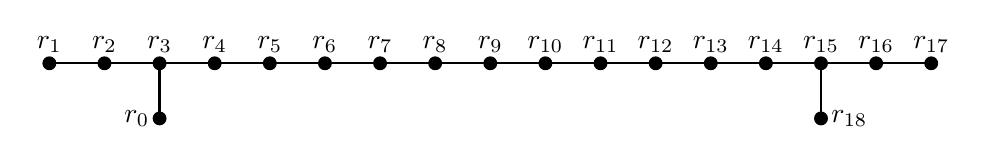
\begin{tikzpicture}[scale=0.7,thick]
\draw (2,0)--(2,1);
\draw (0,1)--(16,1);
\draw(14,0)--(14,1);

\node[above] at (0,1) {$r_1$};
\node[above] at (1,1) {$r_2$};
\node[above] at (2,1) {$r_3$};
\node[above] at (3,1) {$r_4$};
\node[above] at (4,1) {$r_5$};
\node[above] at (5,1) {$r_6$};
\node[above] at (6,1) {$r_7$};
\node[above] at (7,1) {$r_8$};
\node[above] at (8,1) {$r_9$};
\node[above] at (9,1) {$r_{10}$};
\node[above] at (10,1) {$r_{11}$};
\node[above] at (11,1) {$r_{12}$};
\node[above] at (12,1) {$r_{13}$};
\node[above] at (13,1) {$r_{14}$};
\node[above] at (14,1) {$r_{15}$};
\node[above] at (15,1) {$r_{16}$};
\node[above] at (16,1) {$r_{17}$};


\node[left] at (2,0) {$r_0$};
\node[right] at (14,0) {$r_{18}$};

\filldraw[black]
(2,0) circle (3pt)
(14,0) circle (3pt)
(1,1) circle (3pt)
(0,1) circle (3pt)
(2,1) circle (3pt)
(3,1) circle (3pt)
(4,1) circle (3pt)
(5,1) circle (3pt)
(6,1) circle (3pt)
(7,1) circle (3pt)
(8,1) circle (3pt)
(9,1) circle (3pt)
(10,1) circle (3pt)
(11,1) circle (3pt)
(12,1) circle (3pt)
(13,1) circle (3pt)
(14,1) circle (3pt)
(15,1) circle (3pt)
(16,1) circle (3pt)
;

\end{tikzpicture}
\caption{Dual graph of the classes $r_i$.}
\label{fig:dualgraph}
\end{figure}

\begin{figure}
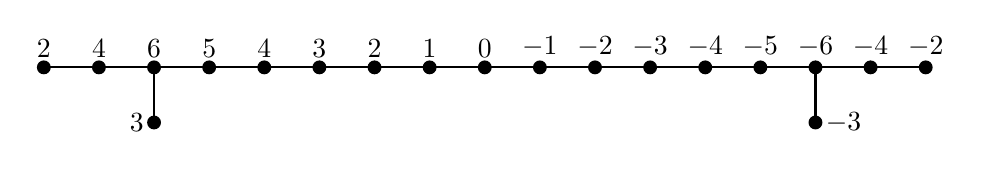
\begin{tikzpicture}[scale=0.7,thick]
\draw (2,0)--(2,1);
\draw (0,1)--(16,1);
\draw(14,0)--(14,1);

\node[above] at (0,1) {$2$};
\node[above] at (1,1) {$4$};
\node[above] at (2,1) {$6$};
\node[above] at (3,1) {$5$};
\node[above] at (4,1) {$4$};
\node[above] at (5,1) {$3$};
\node[above] at (6,1) {$2$};
\node[above] at (7,1) {$1$};
\node[above] at (8,1) {$0$};
\node[above] at (9,1) {$-1$};
\node[above] at (10,1) {$-2$};
\node[above] at (11,1) {$-3$};
\node[above] at (12,1) {$-4$};
\node[above] at (13,1) {$-5$};
\node[above] at (14,1) {$-6$};
\node[above] at (15,1) {$-4$};
\node[above] at (16,1) {$-2$};


\node[left] at (2,0) {$3$};
\node[right] at (14,0) {$-3$};

\filldraw[black]
(2,0) circle (3pt)
(14,0) circle (3pt)
(1,1) circle (3pt)
(0,1) circle (3pt)
(2,1) circle (3pt)
(3,1) circle (3pt)
(4,1) circle (3pt)
(5,1) circle (3pt)
(6,1) circle (3pt)
(7,1) circle (3pt)
(8,1) circle (3pt)
(9,1) circle (3pt)
(10,1) circle (3pt)
(11,1) circle (3pt)
(12,1) circle (3pt)
(13,1) circle (3pt)
(14,1) circle (3pt)
(15,1) circle (3pt)
(16,1) circle (3pt)
;

\end{tikzpicture}
\caption{The class $\xi$.}
\label{fig:Kgraph}
\end{figure}

A discriminant computation shows that the classes $\varphi_X(r_i)$, for $0 \leq i \leq 18$, generate $I^{\perp}/I \cong H \oplus E_8 \oplus E_8$ as a $\bZ$-module. It follows that the $r_i$ form a $\bZ$-basis for $\xi^{\perp}$.

With this description, the lattices $\varphi_X(K_{V_i}^{\perp})$ are as follows.
\begin{itemize}
\item If $K_{V_2}^2 = d \leq 6$, then $\varphi_X(K_{V_1}^{\perp}) = \langle r_0,\ldots,r_{8+d}\rangle \cong E_{9+d}$ and  $\varphi_X(K_{V_2}^{\perp}) = \langle r_{10+d},\ldots,r_{18} \rangle \cong E_{9-d}$. Here we take $E_3 = A_2 \oplus A_1$, $E_4 = A_4$, $E_5 = D_5$, and extend the $E$-series of lattices to $n \geq 9$ in the obvious way.
\item If $K_{V_2}^2 = 8$ and $V_2 \cong \bF_2$, then $\varphi_X(K_{V_1}^{\perp}) = \langle r_0,\ldots,r_{15},r_{18}\rangle \cong E_{17}$ and  $\varphi_X(K_{V_2}^{\perp}) = \langle r_{17} \rangle \cong A_1$.
\end{itemize}

Therefore, given an $H$-polarized Tyurin degeneration of K3 surfaces, to describe the three sublattices $H$ and $\varphi_X(K_{V_i}^{\perp})$ of $I^{\perp}/I$ (up to isometries of $I^{\perp}/I$), it suffices to give the isometry types of the lattices $\varphi_X(K_{V_i}^{\perp})$, as abstract lattices, along with a set of generators for $H$ in terms of the simple roots $r_i \in I^{\perp}/I$ defined above. To denote such generators, we use the following shorthand notation: a class
\[v:= \sum_{i=0}^{18}a_ir_i \in I^{\perp}/I\]
will be denoted by the vector notation
\begin{equation} \label{eq:vectornotation} v = (a_0; a_1,a_2,a_3,a_4,a_5, a_6,a_7,a_8,a_9,a_{10},a_{11},a_{12},a_{13},a_{14},a_{15},a_{16},a_{17};a_{18}).\end{equation}
Note that any such class is only defined modulo 
\[\xi := (3;2,4,6,5,4,3,2,1,0,-1,-2,-3,-4,-5,-6,-4,-2;-3).\]
Then we have the following result.

\begin{proposition}\label{prop:degenerations}
The possible very general $H$-polarized Tyurin degenerations of K3 surfaces, along with the corresponding sublattices $H$ and $\varphi_X(K_{V_i}^{\perp})$ of $I^{\perp}/I \cong H \oplus E_8 \oplus E_8$, are listed in Table \ref{tab:degenerations}. In this table:
\begin{itemize}
\item ``Label'' is the label used to refer to each example in the text.
\item $V_1$ and $V_2$ are the two components of the degenerate fibre $X_0$.
\item $(K_{V_1}^2,K_{V_2}^2)$ gives the self-intersection numbers of the anticanonical classes on each of $V_1$ and $V_2$.
\item  $\varphi_X(K_{V_i}^\perp)$ describes the pair of lattices $(\varphi_X(K_{V_1}^\perp), \varphi_X(K_{V_2}^\perp))$ as abstract lattices. Here we extend the $E_n$-series of lattices to $n \geq 9$ in the obvious way.
\item  ``Generators of $H$'' describes generators of the lattice $H$ in terms of the simple roots $r_i \in I^{\perp}/I$. The notation is described in Equation \eqref{eq:vectornotation}.
\end{itemize} 
Moreover, all of these degenerations are doubly admissible, in the sense of \cite[Definition 3.31]{dfk3slpms}.
\end{proposition}

%\begin{landscape}
%\begingroup
%\renewcommand{\arraystretch}{1.1}
\begin{table}
\begin{tabular}{cccccc}
\hline
\textbf{Label} & $V_1$ & $V_2$ & $(K_{V_1}^2,K_{V_2}^2)$ & $\varphi_X(K_{V_i}^\perp)$ & \textbf{Generators of} $H$\\[.2em]
\hline
\hline 
 \multirow{2}*{$D_{16}$}   & \multirow{2}*{$\mathrm{Bl}_{17}\bP^2$}    & \multirow{2}*{$\bF_2$}  & \multirow{2}*{$(-8,8)$} & \multirow{2}*{$(E_{17},A_1)$}  & $(0;0,0,0,0,0,0,0,0,0,0,0,0,0,0,0,0,1;0)$ \\ 
    &   &  &  &  & $(1;0,1,2,2,2,2,2,2,2,2,2,2,2,2,2,1,0;1)$ \\ 
\hline
 \multirow{4}*{$E_8E_8$}  & \multirow{2}*{$\mathrm{Bl}_{10}\bP^2$}    & \multirow{2}*{$\mathrm{Bl}_{8}\bP^2$} & \multirow{2}*{$(-1,1)$} & \multirow{2}*{$(E_{10},E_8)$}  & $(0;0,0,0,0,0,0,0,0,1,0,0,0,0,0,0,0,0;0)$ \\ 
   &   &  &  &  & $(3;2,4,6,5,4,3,2,1,0,0,0,0,0,0,0,0,0;0)$ \\ 
\cline{2-6}
 & \multirow{2}*{$\mathrm{Bl}_{9}\bP^2$}    & \multirow{2}*{$\mathrm{Bl}_{9}\bP^2$}  & \multirow{2}*{$(0,0)$} & \multirow{2}*{$(E_{9},E_9)$}  & $(0;0,0,0,0,0,0,0,0,1,0,0,0,0,0,0,0,0;0)$ \\ 
   &   &  &  &  & $(0;0,0,0,0,0,0,0,0,0,1,2,3,4,5,6,4,2;3)$ \\ 
\hline
\end{tabular}
\caption{Tyurin degenerations of K3 surfaces.}
\label{tab:degenerations}
\end{table}
%\endgroup
%\end{landscape}

\begin{proof}
We follow the approach from \cite{t2dk3sd4,jonesthesis}. Note that a general $H$-polarized K3 surface may be realised as a double cover of the Hirzebruch surface $\bF_4$ branched over the $(-4)$-section $s$ and a divisor $B$ in the linear system $|3s + 12f|$, where $f$ is the class of a fibre. There are two Type II boundary components in the moduli space of $H$-polarized K3 surfaces \cite[Section 7F]{cmek3sspt}, corresponding to two rank $2$ isotropic sublattices $I \subset H^{\perp}$, which we label by $D_{16}$ and $E_8E_8$, and three easily-observed Tyurin degenerations:

\begin{itemize}
\item \textbf{$D_{16}$ case.} Degenerate $B$ to the union of a double curve in the linear system $|s+4f|$ and a single curve in the linear system $|s+4f|$. The double cover is non-normal over the double curve; blowing this up gives rise to a Tyurin degeneration. The strict transform of the original central fibre is the Hirzebruch surface $V_2 := \bF_2$ and the exceptional component is $V_1 := \mathrm{Bl}_{17}\bP^2$.

\item \textbf{Asymmetric $E_8E_8$ case.} Degenerate $B$ to a curve with a consecutive triple point. The double cover has an elliptic singularity of type $\widetilde{E}_8$ over this point. Performing a weighted blow-up of this point (with weights $(1,1,2,3)$) gives rise to a Tyurin degeneration. The strict transform of the original central fibre is $V_1:= \mathrm{Bl}_{10}\bP^2$  and the exceptional component is $V_2:= \mathrm{dP}_1 = \mathrm{Bl}_{8}\bP^2$.

\item \textbf{Symmetric $E_8E_8$ case.} Degenerate $\bF_4$ to a union $\bF_2 \cup \bF_2$, glued along a fibre of the rulings. The $(-4)$-section degenerates to the union of the two $(-2)$-sections and the branch curve $B$ degenerates to a curve in the linear system $|3s+6f|$ in each component. The double cover is a Tyurin degeneration with both components isomorphic to  $\mathrm{Bl}_{9}\bP^2$.
\end{itemize}

Under the double cover, the classes $s$ and $f$ lift to the classes of a section $S$ and a fibre $F$ of the elliptic fibration on a general $H$-polarized K3 surface; it is straightforward to check that the flat limits $S_0$ and $F_0$ of these two divisors on the central fibre give the stated classes in Table \ref{tab:degenerations}. Note that in the symmetric $E_8E_8$ case we have a choice of which surface to label as $V_1$ and $V_2$; we choose the labelling so that $F_0$ lies in $V_2$.

It remains to prove that there are no further Tyurin degenerations. Following the approach of \cite[Section 5]{t2dk3sd4}, it suffices to compute the wall-and-chamber decomposition on the set of effective lifted polarizations.

Let $\calX \to \Delta$ denote one of the $H$-polarized Tyurin degenerations of K3 surfaces described above. Assume that $\NS(X) \cong H$ for a general fibre $X$ in $\calX$. Then the ample cone of $X$ is bounded by the rays spanned by the classes of $F$ and $S+2F$.

Let $A \subset \calX$ be an effective, flat, and relatively nef and big Cartier divisor, as in the definition of an $H$-polarized Tyurin degeneration, and let $A_0$ be its restriction to $X_0$. The \emph{effective lifts} of $A$ are the set of divisors $A_0 + m \xi$ which are effective on $X_0$, where $m \in \bZ$. The \emph{set of effective lifted polarizations} is the set of all effective lifts.

Any effective lift is linearly equivalent to a divisor on $X_0$ of the form $aS_0 + bF_0 + c \xi$, for some $a,b,c \in \bZ$ and note that each of $S_0$, $F_0$, and $\xi$ is Cartier. Using the description of the divisors $S_0$ and $F_0$  from Table \ref{tab:degenerations} and the description of the ample cone above, we may compute the set of effective lifted polarizations in each case. We note first that the ample cone in $H$ gives the inequalities $a \geq 0$ and $b -2a \geq 0$ in both cases. 
\begin{itemize}[leftmargin=*]
\item \textbf{$D_{16}$ case.} The intersection of $F_0$ with each component of $X_0$ is an irreducible effective divisor of square $0$, so must intersect any other effective divisor non-negatively; this gives the further inequalities $c \geq 0$ and $a - 2c \geq 0$. These four inequalities describe the necessary conditions for an integral class of the above form to be effective. To show these conditions are sufficient, we consider the slice $a+b+c=k$, where $k\in \mathbb{R}$ and demonstrate that classes on the boundary rays are effective. By the convexity of the effective cone, this will provide the necessary and sufficient conditions for a lifted polarization to be effective.

For $k>0$, one can see that these conditions give rise to a triangle in the slice $a+b+c = k$ whose vertices are $(a,b) = (0,k),~ \left(\frac{2k}{7},\frac{4k}{7}\right),~ \left(\frac{k}{3},\frac{2k}{3}\right)$ and by the convexity of the effective cone, it is sufficient to check that the $\mathbb{R}$-divisors corresponding to these vertices are effective. This is straightforward to check: the first and third vertices give effective sums of $S_0$ and $F_0$, and the second vertex gives the effective divisor $\frac{4k}{7}F_0|_{V_1} - \frac{k}{7}K_{V_1}$ on $V_1$ and the zero divisor on $V_2$. Note that when $k=0$, the only class we obtain corresponds to the zero divisor and when $k<0$, the conditions describe the empty set.

\item \textbf{$E_8E_8$ case.} We present the analysis in the symmetric $E_8E_8$ case; the asymmetric case gives rise to the same picture. Each component $V_i$ of $X_0$ is a rational elliptic surface and the sum of a $(-1)$-section and a fibre of the elliptic fibration on $V_i$ is an effective divisor of square $1$, which intersects any other effective divisor non-negatively. This gives the further inequalities $c \geq 0$ and $b \geq c$. We proceed as in the $D_{16}$ case and consider the slice $a+b+c=k$.

For $k>0$, one can see that the conditions give rise to a quadrilateral in the slice $a+b+c = k$ whose vertices are $(a,b) = (0,k),~\left(0,\frac{k}{2}\right), ~\left(\frac{k}{5},\frac{2k}{5}\right),~\left(\frac{k}{3},\frac{2k}{3}\right)$. The first two vertices give rise to multiples of the effective anticanonical divisors $-K_{V_2}$ and $-K_{V_1}$, respectively. The fourth vertex gives $\frac{k}{3}S_0 + \frac{2k}{3}F_0 \sim \frac{k}{3}S_0|_{V_1} - \frac{2k}{3}K_{V_2}$, which is effective, and the third gives the analogous effective $\bR$-divisor $\frac{k}{5}S_0|_{V_2} - \frac{2k}{5}K_{V_1}$, with the labels of the components swapped. As before, this shows that the above conditions are necessary and sufficient conditions for effective lifted polarizations. For $k=0$, we obtain only the zero divisor and for $k<0$ the inequalities describe the empty set.
\end{itemize}

\noindent Within the set of effective lifted polarizations is a subset where the effective lifts are nef on $X_0$. For effective lifted polarizations outside this set, one may flip negative curves between components following the algorithm in the proof of \cite[Theorem 1]{bgd4} to obtain another Tyurin degeneration for which the effective lifted polarization becomes nef. This process endows the set of effective lifted polarizations with a wall-and-chamber structure, in which each chamber corresponds to a Tyurin degeneration and crossing walls corresponds to flipping curves. The argument from the proof of \cite[Theorem 2]{t2dk3sd4} shows that all Tyurin degenerations corresponding to a given Type II boundary component may be obtained in this way. In particular, we exploit the following facts: the nef cone is convex; intersection multiplicities are constant in linear systems; and the only curves which an effective reducible divisor may intersect negatively are its own components, which must necessarily have negative self-intersection.

Performing this analysis for the $H$-polarized degenerations above, we find that the divisors corresponding to the vertices given in the $D_{16}$ case are nef, and hence there is only one chamber in the set of effective lifted polarizations in the $D_{16}$ case. Therefore there is only one Tyurin degeneration in this case.

In the (symmetric) $E_8E_8$ case, the effective lifted polarization intersects a $(-1)$-section of the elliptic fibration on $V_1$ negatively if  $c < a $  and intersects a $(-1)$-section of the elliptic fibration on $V_2$ negatively if $b < a + c$. Flipping either of these sections gives the asymmetric $E_8E_8$ case (possibly with the labels of $V_1$ and $V_2$ switched). Working in a slice $a+b+c=k$, the two inequalities above can be reformulated to say that the conditions $b\geq k/2$ and $2a+b\geq k$ are necessary in order for a divisor to be nef in the symmetric model. This gives rise to a triangle with vertices $(0,k),~\left(0,\frac{k}{2}\right),~ \left(\frac{k}{4},\frac{k}{2}\right)$ and it is easy to check using the above well-known facts that all three of these vertices are nef, therefore this determines the nef cone for the symmetric model. Note that the first vertex intersects the $(-1)$-section on $V_2$ trivially, the second vertex intersects the $(-1)$-section on $V_1$ trivially, and the third vertex intersects both of these $(-1)$-sections trivially. 

Finally, it is easy to check that the only curve which the divisor associated to the vertex $\left(\frac{k}{5},\frac{2k}{5}\right)$ intersects negatively is the $(-1)$-section on $V_2$, hence after flipping this curve to $V_1$, the divisor corresponding to this vertex is a nef divisor on one version of the asymmetric model. Then all the vertices $\left(0,\frac{k}{2}\right),~\left(\frac{k}{5},\frac{2k}{5}\right),~ \left(\frac{k}{4},\frac{k}{2}\right)$ correspond to nef divisors on the asymmetric model and therefore the triangle defined by these points is the nef cone for this version of the asymmetric model. Analogous calculations performed on the vertex $\left(\frac{k}{3},\frac{2k}{3}\right)$ complete the analysis. 

The sets of effective lifted polarizations are depicted in Figure \ref{fig:cones}. In these pictures we depict the slices $a+b+c = 5$, with axes given by $a$ and $b$. The nodes demarcate points where $(a,b)$ are integers and the shaded region is the set of effective lifted polarizations. In the $D_{16}$ case there is only a single chamber. In the $E_8E_8$ case, the dark grey chamber corresponds to divisors which are nef in the symmetric case and the two light grey chambers correspond to divisors which are nef in the asymmetric cases.

\begin{figure}
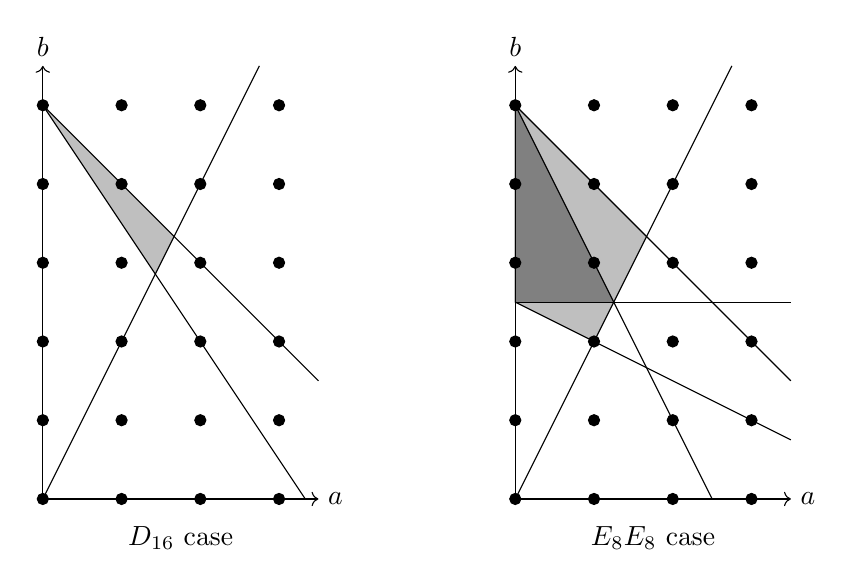
\begin{tikzpicture}
\filldraw[lightgray] (0,5)--(1.4286,2.8571)--(1.6667,3.3333)--(0,5);

\draw[->] (0,0)--(3.5,0);
\draw[->] (0,0)--(0,5.5);
\node[right] at (3.5,0) {$a$};
\node[above] at (0,5.5) {$b$};
\draw (0,0)--(2.75,5.5);
\draw (0,5)--(3.5,1.5);
\draw (0,5)--(3.3333,0);

\filldraw (0,0) circle (2pt);
\filldraw (1,0) circle (2pt);
\filldraw (2,0) circle (2pt);
\filldraw (3,0) circle (2pt);
\filldraw (0,1) circle (2pt);
\filldraw (1,1) circle (2pt);
\filldraw (2,1) circle (2pt);
\filldraw (3,1) circle (2pt);
\filldraw (0,2) circle (2pt);
\filldraw (1,2) circle (2pt);
\filldraw (2,2) circle (2pt);
\filldraw (3,2) circle (2pt);
\filldraw (0,3) circle (2pt);
\filldraw (1,3) circle (2pt);
\filldraw (2,3) circle (2pt);
\filldraw (3,3) circle (2pt);
\filldraw (0,4) circle (2pt);
\filldraw (1,4) circle (2pt);
\filldraw (2,4) circle (2pt);
\filldraw (3,4) circle (2pt);
\filldraw (0,5) circle (2pt);
\filldraw (1,5) circle (2pt);
\filldraw (2,5) circle (2pt);
\filldraw (3,5) circle (2pt);

\node at (1.75,-0.5) {$D_{16}$ case};

\filldraw[lightgray] (6,5)--(6,2.5)--(7,2)--(7.6667,3.3333)--(6,5);
\filldraw[gray] (6,5)--(6,2.5)--(7.25,2.5)--(6,5);

\draw[->] (6,0)--(9.5,0);
\draw[->] (6,0)--(6,5.5);
\node[right] at (9.5,0) {$a$};
\node[above] at (6,5.5) {$b$};
\draw (6,0)--(8.75,5.5);
\draw (6,5)--(9.5,1.5);
\draw (6,2.5)--(9.5,0.75);
\draw (6,2.5)--(9.5,2.5);
\draw (6,5)--(8.5,0);

\filldraw (6,0) circle (2pt);
\filldraw (7,0) circle (2pt);
\filldraw (8,0) circle (2pt);
\filldraw (9,0) circle (2pt);
\filldraw (6,1) circle (2pt);
\filldraw (7,1) circle (2pt);
\filldraw (8,1) circle (2pt);
\filldraw (9,1) circle (2pt);
\filldraw (6,2) circle (2pt);
\filldraw (7,2) circle (2pt);
\filldraw (8,2) circle (2pt);
\filldraw (9,2) circle (2pt);
\filldraw (6,3) circle (2pt);
\filldraw (7,3) circle (2pt);
\filldraw (8,3) circle (2pt);
\filldraw (9,3) circle (2pt);
\filldraw (6,4) circle (2pt);
\filldraw (7,4) circle (2pt);
\filldraw (8,4) circle (2pt);
\filldraw (9,4) circle (2pt);
\filldraw (6,5) circle (2pt);
\filldraw (7,5) circle (2pt);
\filldraw (8,5) circle (2pt);
\filldraw (9,5) circle (2pt);

\node at (7.75,-0.5) {$E_8E_8$ case};
\end{tikzpicture}
\caption{Wall and chamber decompositions of the sets of effective lifted polarizations} \label{fig:cones}
\end{figure}

Finally, we check that these degenerations are doubly admissible. Indeed, the two rank two isotropic sublattices $I \subset H^{\perp} \cong H \oplus H \oplus E_8 \oplus E_8$ correspond to the two embeddings of $H \oplus H$ into $H \oplus H \oplus E_8 \oplus E_8$: the obvious one with orthogonal complement $E_8 \oplus E_8$ and a second with orthogonal complement given by an index $2$ overlattice of $D_{16}$. The doubly admissible condition therefore follows from \cite[Lemma 3.32]{dfk3slpms}.
\end{proof}

\section{Explicit Lattice Computations for Elliptically Fibred Surfaces} \label{sec:ellipticfibrationcomputations}

In this section we present a result that allows for certified computation of the N\'{e}ron-Severi lattice of a generic member of a family of elliptically fibred surfaces, following the approach of \cite{snahlpcesp1}.

We begin with some setup. Let $\pi\colon Y \to \bP^1$ be a relatively minimal elliptically-fibred surface with fixed zero section $S_0$. We consider $H_2(Y;\bZ)$ as a lattice equipped with the usual intersection form. Let $H_{\pi} \subset H_2(Y;\bZ)$ denote the copy of the hyperbolic plane lattice generated by the classes of the zero section $S_0$ and a fibre $F$ and let $R_{\pi} \subset H_2(Y;\bZ)$ denote the sublattice generated by components of fibres that do not meet $S_0$. Following the terminology from \cite{es}, the sublattice $\Trv(Y,\pi) := H_{\pi} \oplus R_{\pi}$ is called the \emph{trivial lattice} in \cite[Definition 7]{snahlpcesp1}.

There is a well known exact sequence of groups
\begin{equation} \label{eq:NSsequence} 0 \longrightarrow \Trv(Y,\pi) \longrightarrow \NS(Y) \longrightarrow \MW(Y,\pi) \longrightarrow 0,\end{equation}
where $\NS(Y)$ denotes the N\'{e}ron-Severi lattice of $Y$ (considered as a sublattice of $H_2(Y;\bZ)$ via Poincar\'{e} duality) and $\MW(Y,\pi)$ denotes the Mordell-Weil group of the elliptic fibration $\pi\colon Y \to \bP^1$, which descends to an exact sequence
\[0 \longrightarrow R_{\pi} \longrightarrow H_{\pi}^{\perp} \longrightarrow \MW(Y,\pi) \longrightarrow 0,\]
where the orthogonal complement $H_{\pi}^{\perp}$ is taken inside $\NS(Y)$ (c.f. \cite[Section VII.2]{btes}).

The relevant results of \cite{snahlpcesp1} may be summarised as follows. Let 
\[\overline{Y} := \{y^2 = x^3 + a(u)x + b(u)\}\]
denote the Weierstrass model of $\pi \colon Y \to \bP^1$, where $u$ is an affine parameter on the base, and assume that the $a(u), b(u) \in \bQ[u]$ are polynomials with rational coefficients. Then \cite{snahlpcesp1} presents a certified algorithm which computes an explicit basis for $H_2(Y;\bZ)$, along with the sublattices $H_{\pi}$ and $R_{\pi}$.

We would like to know the N\'{e}ron-Severi lattice $\NS(Y)$. \cite[Section 4.1]{snahlpcesp1} gives an algorithm to approximate this but, unfortunately, this computation is not certified: in general the result may be larger or smaller than the true N\'{e}ron-Severi lattice.

In this section we present a result to circumvent this problem. Our approach is to realise $Y$ as a special member of an appropriate family of surfaces, then to show that the N\'{e}ron-Severi lattice of a general member is simply the saturation of the trivial lattice, the computation of which is certified. We work under the following assumptions. Let $\pi_t\colon {Y}_t \to \bP^1$ be a smooth family of relatively minimal elliptic surfaces with section, for $t \in \Delta^n$ (the complex polydisc), and let $\overline{Y}_t := \{y^2 = x^3 + a_t(u) x + b_t(u)\}$ be their Weierstrass models. Assume that these satisfy the following.

\begin{assumption} \label{ass:analyticfamily}
\begin{enumerate}
\item $a_t(u)$ and $b_t(u)$ are polynomials in $u$ whose coefficients are holomorphic functions of $t$;
\item $a_0(u), b_0(u) \in \bQ[u]$;
\item for all $t \in \Delta^n$, the elliptic fibrations $\pi_t\colon {Y}_t \to \bP^1$ have the same singular fibre types as $\pi_0\colon Y_0 \to \bP^1$ (equivalently, the covers of $\Delta^n$ defined by the vanishing of $a_t(u)$, $b_t(u)$, and $4a_t(u)^3 + 27b_t(u)^2$ in $\Delta^n \times \bC$ are unramified).
\end{enumerate}
\end{assumption}

%Now follow the algorithm in \cite[Section 4.1]{snahlpcesp1}: numerically approximate the period mapping and let ${N} \subset H_2(Y_0;\bZ)$ denote its kernel. Note that $N$ always contains the trivial lattice $\Trv(Y_0,\pi_0)$. The next result shows that, assuming the Mordell-Weil group is torsion, then the lattice ${N}$ is the N\'{e}ron-Severi lattice of a general member $Y_t$ of the family above.
 The next result shows that, assuming the Mordell-Weil group is torsion, the N\'{e}ron-Severi lattice of a general member $Y_t$ of the family above is simply the saturation of the trivial lattice.

\begin{proposition} \label{prop:torsionMW} Suppose that Assumption \ref{ass:analyticfamily} holds and that $\MW({Y}_t,\pi_t)$ is torsion for very general $t \in \Delta^n$. Then for very general $t \in \Delta^n$, the N\'{e}ron-Severi lattice $\NS({Y}_t)$ is equal to the saturation of $\Trv(Y_0,\pi_0) \cong H_{\pi} \oplus R_{\pi}$ in $H_2(Y;\bZ)$.
\end{proposition}

\begin{proof} Note that, under Assumptions \ref{ass:analyticfamily}, $H_2(Y_t;\bZ)$ are trivial local systems over $\Delta^n$ and the trivial sublattice $\Trv(Y_t,\pi_t)$ varies continuously with $t$, so we may canonically identify $H_2(Y_t;\bZ) \cong H_2(Y_0;\bZ)$ so that $\Trv(Y_t,\pi_t)$ is identified with $\Trv(Y_0,\pi_0)$; we will do this implicitly in the remainder of the proof.

The N\'{e}ron-Severi group of $Y_t$ varies with $t$ and fits into the exact sequence \eqref{eq:NSsequence}. In the case where $\MW({Y}_t,\pi_t) \cong  \NS(Y_t)/\Trv(Y_t,\pi_t)$ is torsion, $\NS(Y_t)$ is just the saturation of $\Trv(Y_t,\pi_t)$ in $H_2({Y}_t;\bZ)$ and so $\NS(Y_t) = {N}$.
\end{proof}

We are interested in $M$-quasipolarized K3 surfaces, in the sense of \cite[Definition 2.6]{cmk3s}, where $M$ denotes the lattice $M := H \oplus E_8 \oplus E_8$. A modular family of $M$-quasipolarized K3 surfaces is described by Clingher and Doran \cite{milpk3s}, based on earlier work of Inose \cite{desk3sni}. This family is dependent upon two parameters $(t_1,t_2)$ (respectively called $(a,b)$ in \cite{milpk3s}). A very general K3 surface in this family admits two elliptic fibrations, called \emph{standard} and \emph{alternate} in \cite{milpk3s}. The standard fibration corresponds to case $E_8E_8$ in Table \ref{tab:Mweierstrass}; its Weierstrass form may be found in \cite[Section 1]{desk3sni}. The alternate fibration corresponds to case $D_{16}$ in Table \ref{tab:Mweierstrass}; its Weierstrass form may be found in \cite[Section 4.4]{milpk3s}. In this table:
\begin{itemize}
\item ``Label'' is the label used to refer to each example in the text.
\item ``Fibres'' is the singular fibre type of a very general member of the family.
\item ``Weierstrass parameters'' are the functions $a_t(u)$ and $b_t(u)$ appearing in the Weierstrass form $y^2 = x^3 + a_t(u)x + b_t(u)$. Here $u$ is an affine parameter on the base $\bP^1$ and $t = (t_1,t_2)$ are deformation parameters.
\item ``MW'' is the Mordell-Weil lattice of a very general member of the family.
\end{itemize}

\begingroup
\renewcommand{\arraystretch}{1.1}
\begin{table}
\begin{tabular}{cccc}
\hline
 \textbf{Label} & \textbf{Fibres} & \textbf{Weierstrass parameters} & \textbf{MW}\\ 
\hline
 \multirow{2}*{$D_{16}$} &  \multirow{2}*{$\rmI_{12}^*\, 6\rmI_1$} & $a_t(u) = u^2(u^6 - \frac{1}{3}(1 - 3t_1u^2 - 2t_2u^3)^2)$ &  \multirow{2}*{$\frac{\bZ}{2 \bZ}$}  \\
  &  & $b_t(u) = \frac{1}{27}u^3(1 - 3t_1u^2 - 2t_2u^3)(2(1 - 3t_1u^2 - 2t_2u^3)^2 - 9u^6)$ &  \\
\hline
 \multirow{2}*{$E_8E_8$} &  \multirow{2}*{$2\rmI\rmI^*\, 4\rmI_1$} & $a_t(u) = -3t_1u^4$ &  \multirow{2}*{$1$}  \\
  &  & $b_t(u) = -u^5(1-2t_2u+u^2)$ &    \\
\hline
\end{tabular}
\caption{Elliptic fibrations on $M$-quasipolarized K3 surfaces.}
\label{tab:Mweierstrass}
\end{table}
\endgroup

These Weierstrass forms satisfy Assumption \ref{ass:analyticfamily} in a neighbourhood of a sufficiently general point $(t_1,t_2) \in \bQ^2$. Given this, explicit computation of the N\'{e}ron-Severi lattices for a very general member of these families may be carried out using Proposition \ref{prop:torsionMW}.

\section{Splittings of elliptic fibrations}\label{sec:splittings}

The setup in this section is taken from \cite[Section 4]{dfk3slpms}. Let $Y$ be an $M$-quasipolarized K3 surface equipped with an elliptic fibration $\pi\colon Y \to \bP^1$ with distinguished zero section $S_0$. Let $\Sigma \subset \bP^1$ denote the finite set of points over which the fibres of $\pi$ are singular.

Let $\gamma \subset \bP^1\setminus \Sigma$ be an allowable loop, in the sense of \cite[Definition 4.11]{dfk3slpms}, and assume that the $M$-quasipolarization is compatible with $\pi$ and $\gamma$, in the sense of \cite[Definition 4.21]{dfk3slpms}. Let $p \in \gamma$ be a point, let $F_p = \pi^{-1}(p)$ denote the fibre over $p$ and let $F$ be its class in $H_2(Y;\bZ)$.  The loop $\gamma$ divides $\bP^1$ into two pieces which are homeomorphic to discs $\Delta_1$ and $\Delta_2$. Let $\pi_1\colon Y_1 \to \Delta_1$ and $\pi_2\colon Y_2 \to \Delta_2$ denote the induced elliptic fibrations over discs. 

Let $\tau \in M^{\perp} \subset H^2(Y;\bZ)$ denote the isotropic class from \cite[Definition 4.21]{dfk3slpms}, obtained by parallel transporting a monodromy invariant cycle in $F_p$ around $\gamma$. Let $\Gamma$ denote the negative definite lattice $\Gamma := F^{\perp}_{M}/\bZ F$, where $F^{\perp}_{M}$ denotes the orthogonal complement of $F$ taken in $M$, and let $J := \bZ F \oplus \bZ \tau \subset H_2(Y;\bZ)$ denote the rank $2$ isotropic sublattice spanned by $F$ and $\tau$. By \cite[Lemma 4.23]{dfk3slpms} we have an embedding $\Gamma \hookrightarrow J^{\perp}/J$ and $J^{\perp}/J \cong H \oplus E_8 \oplus E_8$.

Now let $q \in \gamma$ be another point, let $F_q$ denote the fibre over $q$, and let $U := Y \setminus F_q$. From the Mayer-Vietoris sequence we have an isomorphism
\begin{equation} \label{eq:homologysum} H_2(U,F_p;\bZ) \cong H_2(Y_1,F_p;\bZ) \oplus H_2(Y_2,F_p;\bZ).\end{equation}
There is a boundary map $\phi\colon H_2(U,F_p;\bZ) \to H_1(F_p;\bZ)$ defined by $\phi := \phi_1 - \phi_2$, where $\phi_i\colon H_2(Y_i,F_p;\bZ) \to H_1(F;\bZ)$ is the usual boundary map from the exact sequence of relative homology. 

The relative homology groups $H_2(Y_1,F_p;\bZ)$ are equipped with a (non-symmetric) bilinear form called the \emph{Seifert pairing} \cite[Definition 4.1]{dfk3slpms}. This induces a bilinear form on $\ker(\phi)$ which is symmetric, and hence imbues $\ker(\phi)$ with the structure of a lattice.

From the long exact sequence of relative homology (c.f. \cite[Lemma 4.13]{dfk3slpms}), we have an isomorphism
\[H_2(U;\bZ)/\bZ F \cong \ker(\phi) \subset H_2(U,F_p;\bZ).\]
$H_2(U;\bZ)$ is a lattice when equipped with the topological intersection form and the class $F \in H_2(U;\bZ)$ is totally isotropic, so this bilinear form descends to $H_2(U;\bZ)/\bZ F \cong \ker(\phi)$. By \cite[Proposition 4.18]{dfk3slpms}, this bilinear form on $\ker(\phi)$ is the negative of the one induced by the Seifert pairing. By \cite[Proposition 4.18]{dfk3slpms} there is a surjective map of lattices $\varphi\colon H_2(U;\bZ)/\bZ F  \to F^{\perp}/\bZ F$.

As the loop $\gamma$ is allowable, by \cite[Definition 4.11]{dfk3slpms} there exists a symplectic basis $(a,b)$ for $H_1(F;\bZ)$ such that, for each $i \in \{1,2\}$, the action of anticlockwise monodromy around $\partial \Delta_i$ is given in the basis $(a,b)$ by
\begin{equation}\label{eq:monodromy} \begin{pmatrix} 1 & e(Y_i) - 12 \\ 0 & 1 \end{pmatrix},\end{equation}
where $e(Y_i)$ denotes the topological Euler number of $Y_i$. For each $i \in \{1,2\}$, let $r_i(a)$ denote the class in $H_2(Y_i,F_p;\bZ)$ obtained by parallel transporting $a$ around $\gamma$. The class $r_i(a)$ is isotropic with respect to the Seifert pairing, so we may define a lattice
\begin{align*}\NS(H_2(Y_i,F_p;\bZ)) &:= r_i(a)^{\perp}/r_i(a)\\ 
&= \{v \in H_2(Y_i,F_p;\bZ) \mid \phi_i(v) \text{ is a multiple of } a\}/r_i(a),\end{align*}
where the orthogonal complement $r_i(a)^{\perp}$ is taken with respect to the Seifert pairing.

Let $\Psi \subset H_2(U,F_p;\bZ)$ be the $\bZ$-submodule of rank $2$ generated by the two classes $(r_1(a),0)$ and $(0,r_2(a))$, where these expressions refer to the decomposition \eqref{eq:homologysum}. Then, by \cite[Proposition 4.20]{dfk3slpms}, $\Psi$ is contained in $\ker(\phi) \cong H_2(U;\bZ)/\bZ F$ and there is an exact sequence
\[0 \longrightarrow \bZ \longrightarrow \Psi^{\perp}/\Psi \stackrel{\varphi_Y}{\longrightarrow} J^{\perp}/J \longrightarrow 0,\]
where $\varphi_Y$ is the map induced by $\varphi$ and the orthogonal complement $\Psi^{\perp}$ is taken in $\ker(\phi) \cong H_2(U;\bZ)/\bZ F$. By \cite[Proposition 2.28]{dfk3slpms} there is an inclusion of lattices
\[\Psi^{\perp}/\Psi \subset \NS(H_2(Y_1,F_p;\bZ)) \oplus \NS(H_2(Y_2,F_p;\bZ)).\]

Define classes $r_i(b) \in H_2(Y_i,F_p;\bZ)$, for each $i \in \{1,2\}$, by parallel transporting $b$ around $\partial \Delta_i$. Note that $r_i(b)$ has nontrivial boundary $\phi_i(r_i(b)) = (12 - e(Y_i))a$. As this is a multiple of $a$, $r_i(b)$ descends to a class in $\NS(H_2(Y_i,F_p;\bZ))$; denote this class by $[r_i(b)]$. By \cite[Lemmas 2.32 , 2.33, and Section 4.3]{dfk3slpms}, the classes $[r_i(b)]$ have the following properties:
\begin{itemize}
\item The class $([r_1(b)], -[r_2(b)]) \in  \NS(H_2(Y_1,F_p;\bZ)) \oplus \NS(H_2(Y_2,F_p;\bZ))$ is iso\-tropic and contained in the kernel $\ker(\varphi_Y) \subset \Psi^{\perp}/\Psi$ .
\item For each $i \in \{1,2\}$ we have
\[  (\Psi^{\perp}/\Psi) \cap \NS(H_2(Y_i,F_p;\bZ)) = [r_i(b)]^{\perp}\]
where the orthogonal complement $[r_i(b)]^{\perp}$ is taken in $\NS(H_2(Y_i,F_p;\bZ))$. Combined with the fact that
\[\Psi^{\perp} \subset \ker(\phi) \subset H_2(Y_1,F_p;\bZ) \oplus H_2(Y_2,F_p;\bZ),\]
and the definition of $\NS(H_2(Y_i,F_p;\bZ))$, it follows that
\begin{equation} \label{eq:ribperp} [r_i(b)]^{\perp} = (\Psi^{\perp} \cap H_2(Y_i,F_p;\bZ))/\bZ r_i(a).\end{equation}
\item The map $\varphi_Y$ is injective on $[r_i(b)]^{\perp}$, for each $i \in \{1,2\}$.
\end{itemize}

It follows that we have three sublattices of $J^{\perp}/J \cong H \oplus E_8 \oplus E_8$:
\begin{itemize}
\item The lattice $\Gamma := F^{\perp}_{M}/\bZ F$;
\item The lattices $\varphi_Y([r_i(b)]^{\perp})$, for $i \in \{1,2\}$.
\end{itemize}

The aim of the rest of this section is to compute simple loops $\gamma$ for the elliptic fibrations from Table \ref{tab:Mweierstrass}, verify that they are allowable and compatible with the $M$-quasipolarization, check that the polarizations are doubly admissible (in the sense of \cite[Definition 4.29]{dfk3slpms}), and explicitly compute the three lattices $\Gamma$, $\varphi_Y([r_1(b)]^{\perp})$ and $\varphi_Y([r_2(b)]^{\perp})$.

To do this we use the following method.
\begin{enumerate}
\item Let $\pi\colon Y \to \bP^1$ be one of the elliptic fibrations from Table \ref{tab:Mweierstrass}. Fix a point $(t_1,t_2) \in \bQ^2$ around which Assumption \ref{ass:analyticfamily} holds; we chose the point $(-3,7)$. We then applied the algorithm from \cite{snahlpcesp1} (which is implemented in SageMath \cite{sage}) to compute an explicit basis for the lattice $H_2(Y;\bZ)$, along with the sublattices $H_{\pi}$ and $R_{\pi}$ with respect to this basis. $R_{\pi}$ is isometric to $E_8 \oplus E_8$ in the $E_8E_8$-fibration and $D_{16}$ in the $D_{16}$-fibration; it is straightforward to check that the saturation of $\Trv(Y,\pi) = H_{\pi} \oplus R_{\pi}$ in $H^2(Y;\bZ)$ is equal to $M$.
\item Use linear algebra to compute an explicit basis for $H^{\perp}_{\pi} \subset H_2(Y;\bZ)$ and express the bilinear form in this basis. As there is a unique embedding $H \subset \Lambda_{\rmK 3}$ up to isometry \cite[Proposition 1.6.1]{isbfa}, $H^{\perp}_{\pi}$ will be isometric to $H \oplus H \oplus E_8 \oplus E_8$.  The composition $H_{\pi}^{\perp} \hookrightarrow F^{\perp} \to F^{\perp}/\bZ F$ is an isometry of lattices, so we may identify $H_{\pi}^{\perp} \cong F^{\perp}/\bZ F$.
\item Part of the algorithm from \cite{snahlpcesp1} computes the action of monodromy around simple loops around each singular fibre in $\pi\colon Y \to \bP^1$, with respect to a base point $p \in \bP^1 \setminus \Sigma$. We ran a brute-force search over concatenations of these loops, looking for classes of simple loops $\gamma$ in $\pi_1(\bP^1 \setminus \Sigma,p)$ for which the monodromy condition \cite[Assumption 4.9(1)]{dfk3slpms} holds. Up to symmetry, this process returned one loop in the $D_{16}$-fibration, which splits the fibration into $Y_1$ containing fibres of types $\rmI_{12}^*\,  2\rmI_1$ and $Y_2$ containing $4\rmI_1$. In the $E_8E_8$-fibration, the process returned two loops, which split the fibration into $Y_1$ containing fibres of types $\rmI\rmI^*\, 3\rmI_1$ (respectively  $\rmI\rmI^*\, 2\rmI_1$) and $Y_2$ containing $\rmI\rmI^*\, \rmI_1$ (respectively  $\rmI\rmI^*\, 2\rmI_1$).
\item Part of the algorithm from \cite{snahlpcesp1} computes an explicit basis for $H_2(U,F_p;\bZ)$, which splits into a direct sum of relative homology groups $H_2(Y_i,F_p;\bZ)$ by Equation \eqref{eq:homologysum}. For each loop $\gamma$ found in the previous step, we used this to find explicit bases for $H_2(Y_i,F_p;\bZ)$, for each $i \in\{1,2\}$, and to compute the classes $r_i(a)$ in those bases. We then checked that $r_i(a)$ is primitive in $H_2(Y_i,F_p;\bZ)$, for each $i \in \{1,2\}$. This verifies \cite[Assumption 4.9(2)]{dfk3slpms} and hence proves that the loop $\gamma$ is allowable \cite[Definition 4.11]{dfk3slpms}.
\item Using linear algebra, compute a basis for $\ker(\phi) \subset H_2(Y_1,F_p;\bZ) \oplus H_2(Y_2,F_p;\bZ)$, in terms of the bases from step (4).
\item Composing the map $\varphi$ with the isomorphism $F^{\perp}/\bZ F \cong H_{\pi}^{\perp}$ gives a surjective map
\[\overline{\varphi}\colon \ker(\phi) \longrightarrow H_{\pi}^{\perp}\]
Compute this map explicitly in terms of the bases from steps (2) and (5).
\item $\overline{\varphi}$ takes the generators $(r_1(a),0)$ and $(0,r_2(a))$ of $\Psi$ to the class $\tau$. Compute this class $\tau$ in the basis for $H_{\pi}^{\perp}$ from step (2). Check that $\tau$ is contained in the orthogonal complement $R_{\pi}^{\perp}$. As $M$ is the saturation of $\Trv(Y,\pi) = H_{\pi} \oplus R_{\pi}$, this verifies that $\tau \in M^{\perp}$, thereby showing that the $M$-quasipolarization is compatible with $\pi$ and $\gamma$ \cite[Definition 4.21]{dfk3slpms}.
\item Check $\tau$ is $1$-admissible in $M^{\perp}$ by finding a class $g \in M^{\perp}$ such that $\tau$ and $g$ generate a copy of the hyperbolic plane lattice. Denote the lattice generated by $\tau$ and $g$ by $H_{\tau}$; note that $H_{\tau} \subset H_{\pi}^{\perp}$. By \cite[Proposition 4.30]{dfk3slpms}, this proves that the $M$-quasipolarization is doubly admissible.
\item Using linear algebra, compute an explicit basis for $J_{\tau} := (H_{\pi} \oplus H_{\tau})^{\perp} \subset H_2(Y;\bZ)$ and express the bilinear form in this basis. As there is a unique embedding $H \oplus H \subset \Lambda_{\rmK 3}$ up to isometry \cite[Proposition 1.6.1]{isbfa}, $J_{\tau}$ will be isometric to $H \oplus E_8 \oplus E_8$. It follows from \cite[Lemma 5.4]{mslpk3s} that we may decompose
\[H_2(Y;\bZ) = H_{\pi} \oplus H_{\tau} \oplus J_{\tau},\]
from which it follows that there is an isometry $J_{\tau} \cong J^{\perp}/J$.
\item Explicitly compute $\Gamma := M \cap J_{\tau}$. By construction, we will have $\Gamma \cong F^{\perp}_{M}/\bZ F$.
\item Compute $\Psi^{\perp} \cap H_2(Y_i,F_p;\bZ)$ in terms of the basis of $\ker(\phi)$ from step (5), where the orthogonal complement $\Psi^{\perp}$ is taken in $\ker(\phi)$. Using step (6), compute $\overline{\varphi}(\Psi^{\perp} \cap H_2(Y_i,F_p;\bZ)) \subset H_{\pi}^{\perp}$.  Finally, compute $\overline{\varphi}(\Psi^{\perp} \cap H_2(Y_i,F_p;\bZ)) \cap J_{\tau}$;  by Equation \eqref{eq:ribperp}, this will equal $\varphi_Y([r_i(b)]^{\perp})$.
\end{enumerate}

\begin{remark}
For the loop which splits the $E_8E_8$-fibration into two pieces which each contain $\rmI\rmI^*\, 2\rmI_1$ fibres, the class $a \in H_1(F_p;\bZ)$ from step (4) will be non-unique, as in this case there is more than one choice of monodromy invariant cycle, and thus there will also be more than one possibility for the class $\tau$. In this case, steps (7) and (8) provide constraints on the possible $a$'s that can be chosen.
\end{remark}

Note that the computations above take place on the K3 surface $Y$ corresponding to $(t_1,t_2) = (-3,7)$ but, by Proposition \ref{prop:torsionMW}, the lattice $M \subset H_2(Y;\bZ)$ found in Step (1) is only known to be equal to the N\'{e}ron-Severi lattice for a very general member of the corresponding family of K3 surfaces. The following lemma shows that the computation above extends to a neighbourhood of this point, so gives the correct lattices $\Gamma$, $\varphi_Y([r_1(b)]^{\perp})$ and $\varphi_Y([r_2(b)]^{\perp})$ for a very general member of the family.

\begin{lemma} \label{lem:deformation} There exists an open (analytic) neighbourhood $U$ of $(t_1,t_2) = (-3,7)$ such that, for very general $t \in U$, we have $\NS(Y_t) \cong M$  and the algorithm above computes $\Gamma$, $\varphi_{Y_t}([r_1(b)]^{\perp})$ and $\varphi_{Y_t}([r_2(b)]^{\perp})$.
\end{lemma}

\begin{proof} The fact that $\NS(Y_t) \cong M$ for very general $t \in U$ follows from Proposition \ref{prop:torsionMW}. Recall that $\Sigma \subset \bP^1$ denotes the set of points over which the fibres of $\pi\colon Y \to \bP^1$ are singular. Let $\delta > 0$ and let 
\[\Sigma_{\delta} := \{x \in \bP^1 : | x - s| < \delta \text{ for some } s \in \Sigma\}\]
be a $\delta$-neighbourhood of $\Sigma$. Choose $\delta > 0$ sufficiently small such that $\Sigma_{\delta}$ does not intersect the loop $\gamma$ and each connected component of $\Sigma_{\delta}$ contains precisely one point from $\Sigma$. 

As the singular fibre type of ${Y}_t$ is independent of $t$ and the singular fibres occur at roots of the discriminant $4a_t(u)^3 + 27b_t(u)^2$, which is a polynomial in $u$ that varies holomorphically with $t$,  we may find a neighbourhood $U$ of $t=(-3,7)$ such that for all $t \in U$, the singular fibres of ${Y}_t$ occur over points in $\Sigma_{\delta}$. Then the loops $\gamma$ found in step (3) of the algorithm above satisfy the required monodromy properties for all $t \in U$ and the groups $H_2(({Y}_t)_i,F_p;\bZ)$ are independent of $t$. The remaining computations find continuously varying classes/sublattices in the trivial local systems $H_2(({Y}_t)_i,F_p;\bZ)$ and $H_2({Y}_t;\bZ)$, so are independent of $t$.
\end{proof}

We thus obtain the following.

\begin{proposition}\label{prop:splittings}
There exist allowable splitting loops on the elliptic fibrations from Table \ref{tab:Mweierstrass} which are compatible with the $M$-quasipolarizations, as listed in Table \ref{tab:splittingdata}. All of them are doubly admissible. In this table:
\begin{itemize}
\item ``Label'' is the label used to refer to each example in the text.
\item ``Splittings'' describes the singular fibre types on either side of the allowable loop; the loop is represented by a vertical bar $|$. We label the pieces of the splitting so that $Y_1$ contains the fibres listed to the left of the bar and $Y_2$ contains those listed to the right.
\item ``Monodromy'' gives the values $(e(Y_1) - 12, e(Y_2)-12)$ in the monodromy matrix from Equation \eqref{eq:monodromy} on each side of the loop.
\item  $\varphi_Y([r_i(b)]^{\perp})$ describes the pair of lattices $(\varphi_Y([r_1(b)]^{\perp}), \varphi_Y([r_2(b)]^{\perp}))$ as abstract lattices. Here we extend the $E_n$-series of lattices to $n \geq 9$ in the obvious way.
\item $\Gamma$ gives the isometry type of the lattice $\Gamma$, as an abstract lattice. Here $D_{16}^+$ is an index $2$ overlattice of the negative definite $D_{16}$ root lattice.
\end{itemize}
\end{proposition}

\begin{table}
\begin{tabular}{ccccc}
\hline
 \textbf{Label} & \textbf{Splittings} & \textbf{Monodromy} & $\varphi_Y([r_i(b)]^{\perp})$ & $\Gamma$\\ 
\hline
 $D_{16}$ & $\rmI_{12}^*\,  2\rmI_1\, |\, 4\rmI_1$ & $(8, -8)$ & $(E_{17}, A_1)$ & $D_{16}^+$\\
\hline
\multirow{2}*{$E_8E_8$} &  $\rmI\rmI^*\, 3\rmI_1 \, |\, \rmI\rmI^*\, \rmI_1$ & $(1,-1)$ & $(E_{10}, E_8)$ & $E_8\oplus E_8$\\
 & $\rmI\rmI^*\, 2\rmI_1 \, |\, \rmI\rmI^*\, 2\rmI_1$ & $(0,0)$& $(E_{9}, E_9)$ & $E_8\oplus E_8$\\
\hline
\end{tabular}
\caption{Splitting data.}
\label{tab:splittingdata}
\end{table}

\begin{remark} Step (3) in the method above was carried out by searching over words in the fundamental group up to a prescribed length, whose letters are simple loops around one singular fibre. We therefore cannot guarantee that we have found \emph{all} possible allowable splittings of the elliptic fibrations from Table \ref{tab:Mweierstrass}, although we expect this to be the case. \end{remark}

\section{Mirror symmetry}

\begin{theorem}\label{thm:mirror}
Given a very general $H$-polarized Tyurin degeneration of K3 surfaces $\calX \to \Delta$, there exists an elliptic fibration $\pi\colon Y \to \bP^1$  on a very general $M$-quasi\-polarized  K3 surface $Y$ and an allowable loop $\gamma \subset \bP^1$, such that the $M$-quasipolarization is compatible with $\pi$ and $\gamma$, so that $\calX \to \Delta$ and $\pi\colon Y \to \bP^1$ form a mirror pair in the sense of \cite[Definition 5.1]{dfk3slpms}.
\end{theorem}

\begin{proof}
As all of the degenerations found in Proposition \ref{prop:degenerations} are doubly admissible, to check that such a degeneration $\calX \to \Delta$ and a fibration $\pi\colon Y \to \bP^1$ with splitting form a mirror pair, by \cite[Proposition 5.3]{dfk3slpms} it suffices to check that there is an isometry $\psi\colon J^{\perp}/J \to I^{\perp}/I$ such that $\psi(\Gamma) = H^{\perp}$ and $\psi(\varphi_Y([r_i(b)]^{\perp})) = \varphi_X(K_{V_i}^{\perp})$ for each $i \in \{1,2\}$.

The matching between Tyurin degenerations and fibrations is simply given by comparing rows in Tables \ref{tab:splittingdata} and \ref{tab:degenerations} (noting that mirror symmetry predicts that $e(Y_i) - 12 = -K_{V_i}^2$).  The sublattices $\Gamma$ and $\varphi_Y([r_i(b)]^{\perp})$ of $J^{\perp}/J \cong H \oplus E_8 \oplus E_8$ are computed explicitly in Section \ref{sec:splittings} and the sublattices $H$ and $\varphi_X(K_{V_i}^\perp)$ of $I^{\perp}/I \cong H \oplus E_8 \oplus E_8$ are computed explicitly in Proposition \ref{prop:degenerations}, so to prove the final part it suffices to find an isometry of $H \oplus E_8 \oplus E_8$ matching the two in each case. 

In the $E_8E_8$ case, we begin by mapping the classes $r_0,\ldots,r_7 \in I^{\perp}/I$ to generators of $\Gamma \cap \varphi_Y([r_1(b)]^{\perp}) \cong E_8$ and $r_{11},\ldots,r_{18} \in I^{\perp}/I$ to generators of $\Gamma \cap \varphi_Y([r_2(b)]^{\perp}) \cong E_8$; there are finitely many ways to do this, corresponding to isometries of the $E_8$ lattice. Combining these maps gives an isometry between $H^{\perp}$ and $\Gamma$, which are both isometric to $E_8 \oplus E_8$. Each such map admits four lifts to an isometry from $I^{\perp}/I$ to $J^{\perp}/J$, corresponding to the four isometries of $H \cong \Gamma^{\perp}$. A brute force computer search is then used to find such an isometry which takes $\varphi_X(K_{V_i}^{\perp})$ to $\varphi_Y([r_i(b)]^{\perp})$ for each $i \in \{1,2\}$.

In the $D_{16}$ case, we begin by mapping the classes $r_0,r_2,r_3,\ldots,r_{15},r_{18} \in I^{\perp}/I$ to generators of $\Gamma \cap \varphi_Y([r_1(b)]^{\perp}) \cong D_{16}$; there are finitely many ways to do this, corresponding to isometries of the $D_{16}$ lattice. Half of these maps lift to isometries between $H^{\perp}$ and $\Gamma$, which are both isometric to an index $2$ overlattice of $D_{16}$. Each such lift admits four further lifts to an isometry from $I^{\perp}/I$ to $J^{\perp}/J$, corresponding to the four isometries of $H \cong \Gamma^{\perp}$. A brute force computer search is then used to find such an isometry which takes $\varphi_X(K_{V_i}^{\perp})$ to $\varphi_Y([r_i(b)]^{\perp})$ for each $i \in \{1,2\}$.
\end{proof}

\textbf{Data access statement.} SageMath notebooks containing code reproducing all computations in this paper will be made available at \cite{Hpolcode}.

\bibliography{publications,preprints}
\bibliographystyle{amsalpha}
\end{document}
